%%%%%%%%%%%%%%%%%%%%%%%%%%%%%%%%%%%%%%%%%%%%%%%%%%%%%%%%%%%%%%%%%%%%%%%% 
%%%%%%%%%%%%%%%%%%%%%%%%%%%%%%%%%%%%%%%%%%%%%%%%%%%%%%%%%%%%%%%%%%%%%%%% 
\begin{frame}
  \frametitle{The future of portable asynchonous tasking}

  {\large \textcolor{darkgreen}{{\bf HiHAT initiative:} Hierarchical Heterogenous Asynchronous Tasking}}

  \begin{itemize}
  \item for Runtime frameworks developpers + HW vendors
  \item<1> Tasking frameworks
  \item<2> Fonctionalities
  \end{itemize}
  
  \only<1>{
    \begin{center}
      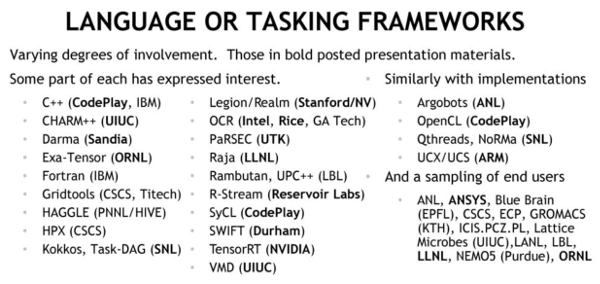
\includegraphics[height=5.0cm]{doc/perf_portability/hihat/hihat_1b}
    \end{center}
  }
  \only<2>{
    \begin{center}
      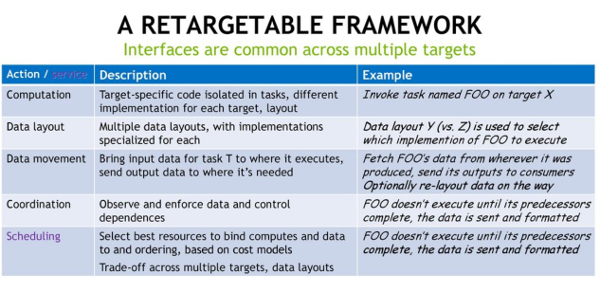
\includegraphics[height=5.0cm]{doc/perf_portability/hihat/hihat_2b}
    \end{center}
  }

  {\small
    reference \myhref{https://wiki.modelado.org/images/5/54/HiHAT_Mini-Summit_17_Overview.pdf}{HiHAT\_Mini-Summit\_17\_Overview.pdf}\\
    reference \myurl{http://slideplayer.com/slide/12990108/}
  }

\end{frame}

%%%%%%%%%%%%%%%%%%%%%%%%%%%%%%%%%%%%%%%%%%%%%%%%%%%%%%%%%%%%%%%%%%%%%%%% 
%%%%%%%%%%%%%%%%%%%%%%%%%%%%%%%%%%%%%%%%%%%%%%%%%%%%%%%%%%%%%%%%%%%%%%%% 
\begin{frame}
  \frametitle{AMT : Asynchonous Many Task frameworks}
  
  \begin{itemize}
  \item \myhref{https://github.com/StanfordLegion/legion}{Legion} (Stanford, C++ Runtime, Regent/language, data partioning)
  \item \myhref{http://starpu.gforge.inria.fr/}{StarPU} (Inria Bordeaux, graph of tasks, runtime task scheduling, data dependecies $\Rightarrow$ task dependencies)
  \item \myhref{https://share-ng.sandia.gov/darma/}{DARMA} (Sandia NL, Async. Many Task programing, abstraction between applications and and low-level runtime scheduling)
    %\myurl{http://theory.stanford.edu/~aiken/WEST/Talks/Darma.pdf}\\
    %\myurl{https://indico.sissa.it/event/8/contribution/64/material/slides/0.pdf}
    %\myurl{https://share-ng.sandia.gov/darma/_assets/documents/ECP-Review-2016-DARMA.pdf}
  \item \myhref{http://charmplusplus.org/}{Charm++} (Univ. Illinois, Urbana Champain, implements a distributed adaptive runtime system, age > 15 years)
  \item \myhref{http://uintah.sci.utah.edu/}{Uintah}, (DAG task graph-based computational framework, PDE solving on structured adaptive grids, scalable IO PIDX, GPU)
    % couplage Kokkos possible
    % https://extremecomputingtraining.anl.gov/files/2014/01/ARGONNEDOEforPDF.pdf
    % http://www.sci.utah.edu/publications/Hol2017b/pearc17.pdf
  \item \myhref{https://github.com/STEllAR-GROUP/hpx}{HPX} (LSU, general purpose C++ runtime system for parallel and distributed applications)
  \item \myhref{https://www.khronos.org/sycl}{SYCL} (cross-platform asynchronous task graph, C++/OpenCL, no distributed parallelism yet)
  \item \myhref{http://icl.cs.utk.edu/parsec/}{ParSEC/PLASMA} (U. Tennessee, architecture aware scheduling of micro-task on heterogenous hardware, linear algebra applications)
  \item \myhref{http://www.dash-project.org/}{DASH} (distributed data struct. + C++/template PGAs)
  \end{itemize}

  {\small
    others runtime systems: \myurl{https://hihat-wiki.modelado.org/Runtime_Clients}\\
    \myhref{https://share-ng.sandia.gov/darma/_assets/documents/Sandia2015_AMT_RTS_L2.pdf}{Comparative analysis of Legion, Charm++, Uintah}
  }

  % preliminaires ?
  % https://github.com/ecrc/hicma
  
\end{frame}
